\documentclass[english, paper]{mmt} % use for seminar paper

\usepackage{mathptmx}
\usepackage{graphicx}
\usepackage{times}
\usepackage{subfig}
\usepackage{float}
\usepackage[utf8]{inputenc}
\usepackage{listings}
\usepackage{makecell}
\usepackage[toc,page]{appendix}
\usepackage{hyperref}
\hypersetup{
    colorlinks,
    citecolor=black,
    filecolor=black,
    linkcolor=black,
    urlcolor=black
}
\usepackage{breakurl}

\usepackage{amsmath}
\usepackage[autostyle,german=guillemets]{csquotes}

\usepackage{verbatim}
\usepackage{setspace}
\usepackage{parskip}
\onehalfspacing

\newcommand{\detailtexcount}[1]{%
  \immediate\write18{texcount -merge -sum -q #1.tex > #1.wcdetail }%
  \verbatiminput{#1.wcdetail}%
}


\usepackage{abbrevs}
%% the following solves a bug in the abbrevs package, that adds an empty
%% space after the abbrev
\makeatletter
\renewcommand\maybe@space@{%
  % \@tempswatrue % <= this is in the original
  \maybe@ictrue % <= this is new
  \expandafter   \@tfor
    \expandafter \reserved@a
    \expandafter :%
    \expandafter =%
                 \nospacelist
                 \do \t@st@ic
  % \if@tempswa % <= this is in the original
  \ifmaybe@ic % <= this is new
    \space
  \fi
}
\makeatother
%%

\usepackage[style=ieee,maxbibnames=2,minbibnames=1,maxcitenames=2,mincitenames=1, backend=biber]{biblatex}
\bibliography{bibliography.bib}

\lstset{ 
  numbers=left,
  literate=%
    {Ö}{{\"O}}1
    {Ä}{{\"A}}1
    {Ü}{{\"U}}1
    {ß}{{\ss}}1
    {ü}{{\"u}}1
    {ä}{{\"a}}1
    {ö}{{\"o}}1
    {~}{{\textasciitilde}}1
}

%% Add configuration options
\newabbrev{\authornamea}{Fabian Cordt}
\newabbrev{\authormaila}{fcordt.itsb-b2021@fh-salzburg.ac.at}
\newabbrev{\authorinsta}{FH Salzburg}
\newabbrev{\authornameb}{Elisabeth Gisser}
\newabbrev{\authormailb}{egisser.itsb-b2022@fh-salzburg.ac.at}
\newabbrev{\authorinstb}{FH Salzburg}
\newabbrev{\authornamec}{Michael Hofreiter}
\newabbrev{\authormailc}{mhofreiter.itsb-b2021@fh-salzburg.ac.at}
\newabbrev{\authorinstc}{FH Salzburg}
\newabbrev{\titlename}{Data Modeller ITS Project}
\newabbrev{\subtitlename}{ITS-Bahn}


%% Paper title.

\title{\titlename \\ \large \subtitlename}

%% This is how authors are specified in the conference style

%% Author 
\author{
	\authornamea\\ \tiny \authormaila 
	\\ \tiny \authorinsta
	\and
	\authornameb\\ \tiny \authormailb 
	\\ \tiny \authorinstb
	\and
	\authornamec\\ \tiny \authormailc
	\\ \tiny \authorinstc
}

\newcommand{\printbibliographyiee}{\begin{singlespace}\printbibliography\end{singlespace}}

\begin{document}
\selectthesislanguage

\pagenumbering{gobble}

\begingroup 
% is required because paper template messes with sizes
\fontsize{12}{18}\selectfont        
\setlength{\parindent}{0pt}
\setlength{\parskip}{5pt plus 2pt minus 1pt}
\sectionfont{\fontsize{14}{15}\selectfont}    

    \onecolumn           
    
    \pagenumbering{roman}

\endgroup


\mmtcolumnmode % switch back to column formatting of stylesheet

\maketitle % used for paper formatting

\pagenumbering{arabic}


%for reference to this section
\section{Beschreibung}
\label{section:Beschreibung}

Generell sollte das Model selbsterklärend sein, der Großteil der Beziehungen konnte direkt aus den Angaben ausgelesen werden. 
Es folgt eine kurze Beschreibung der wichtigsten Entitätsgruppen und Beziehungen:

\begin{description}
    \item[Zug, Wagon und Lokomotive] Der Zug und seine verknüpften Entitäten wurden aus der Angabe ausgelesen. 
    Klasse, Zugtyp, Wagontyp und Lokomotivtyp wurden als eigene Tabellen normiert. 
    Dies hat den Vorteil, dass diverse Preisinformationen ohne Redundanz verknüpft werden können.
    \item[Fahrplan und Strecke] Eine Strecke wurde als Summe von Streckenabschnitten (verknüpft mit einem Fahrplan) realisiert.
    Jeder Streckenabschnitt hat einen Abfahrtsbahnsteig (mit Uhrzeit), und einen Ankunftsbahnsteig (ebenfalls mit Uhrzeit). 
    Der Start eines Fahrplans ist der Abfahrtsbahnsteig jenes Streckenabschnitts, der die geringste Uhrzeit hat, 
    und das Ende eines Fahrplans ist, komplementär, der Ankunftsbahnsteig jenes Streckenabschnitts, der die höchste Uhrzeit hat.
    \item[Bahnhof] Der Bahnhof ist selbsterklärend: Jeder Bahnhof besitzt mindestens einen Bahnsteig. 
    Der Ort eines Bahnhofs wurde als eigene Tabelle normiert, da auch eine Kundin einem Ort zugeteilt ist.
    \item[Ticket] Die Tickets wurden als ein hierarchisches Vererbungsmodell realisiert. Jedes Ticket hat eine Nummer und ein Gültigkeitsdatum.
    Einem Dauerticket ist dabei eine Kundin zugeordnet. Zusätzlich hat das Dauerticket einen Dauertyp (Jahr, Monat, Woche), 
    der zusätzlich zum Gültigkeitsdatum (``Startdatum'') das Ende des Dauertickets bestimmt.
    Einer anonymen Einzelfahrt sind zwei Bahnsteige zugeordnet (``von'', ``bis'').
    Hat der Kunde eine Sitzplatzreservierung erstanden, so ist auch ein eindeutiger Sitzplatz dem Ticket zugewiesen.
    Die Beziehung zwischen Sitzplatz und Einzelfahrt mit Reservierung ist eine 1:N, da ein Sitzplatz zu verschiedenen Zeiten 
    von verschiedenen Kunden reserviert werden kann.
    \item[Preis] Die verschiedenen Preise (``Preis je Haltestelle'', ``Dauerticketpreis'', ``Einzelticketpreis'' und ``Reservierungsaufschlag'') 
    sind mit den relevanten Tabellen verknüpft. Zusätzlich hat jeder Preis ein Gültigkeitsdatum (``von'', ``bis''). 
    Damit können Preiserhöhungen schon im Vorfeld in das Datenmodell eingetragen werden, und haben erst ab einem bestimmten Tag eine Auswirkung auf die Ticketpreise.
\end{description}
\begin{figure}[h]
    \caption{Logisches Modell}
    \centering
    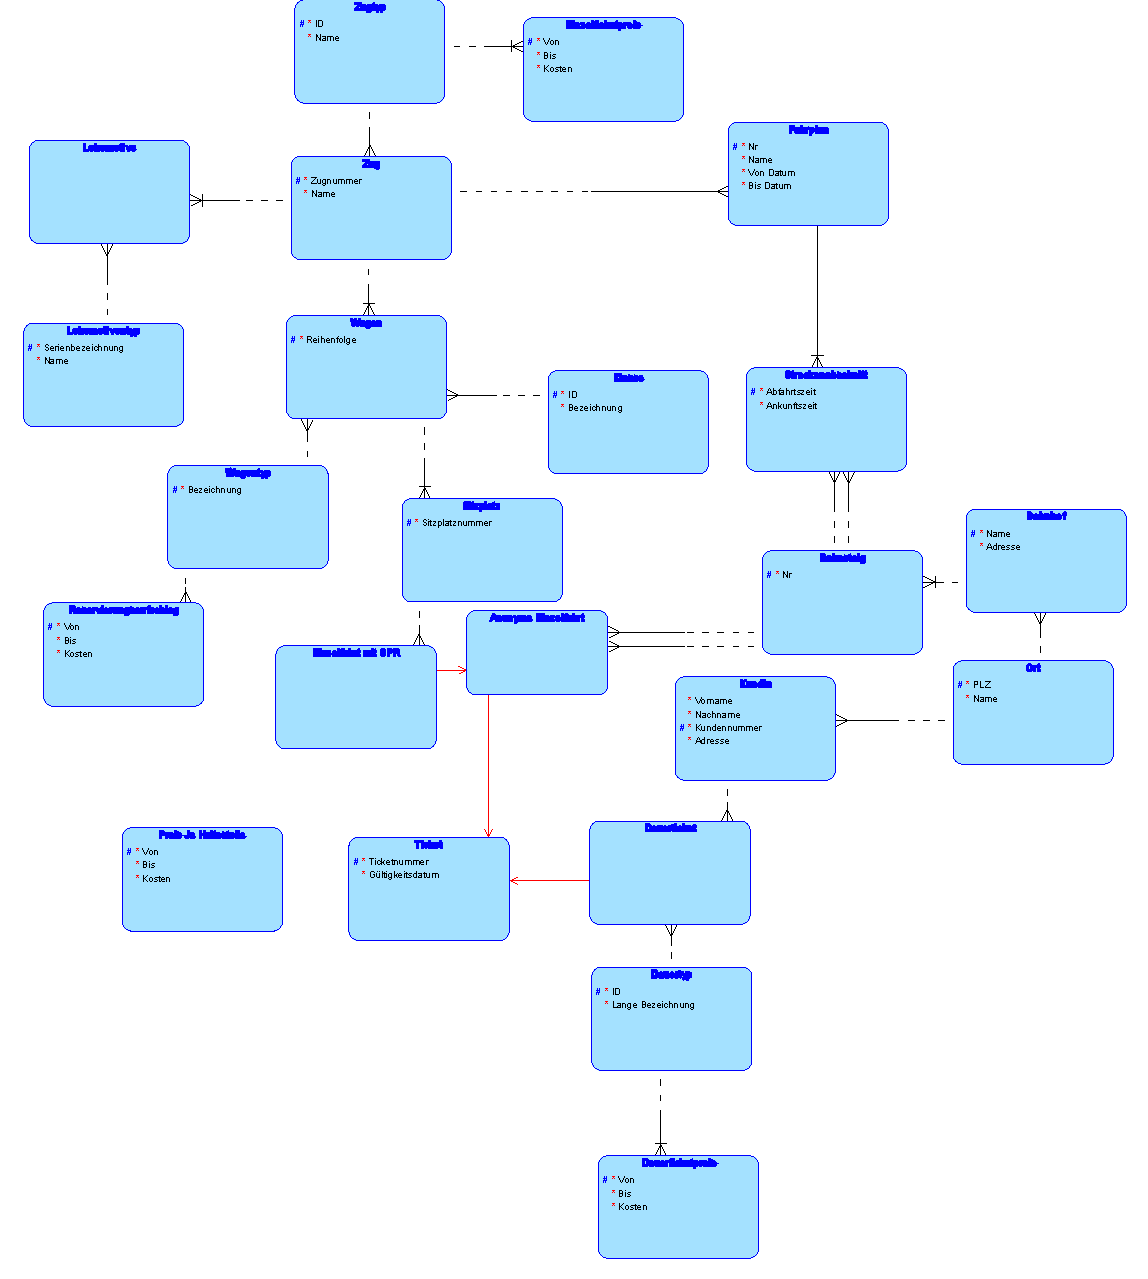
\includegraphics[width=1\textwidth]{logical}
\end{figure}\label{diagramm}
\section{Diagramm}
\label{section:Diagramm}

In \ref{diagramm} ist das logische Modell zusehen, in \ref{sec:ddl} ist das SQL Script zu sehen, dass zur Erstellung
des Datenmodells in der Datenbank benutzt wurde. Es fehlen noch die Sequenzes für gewisse
Tabellen (im Speziellen \texttt{TICKET.TICKERNUMMER}, und \texttt{KUNDIN.KUNDENNUMMER}.)
\section{Befüllen der Datensätze}
Das Befüllen der Datensätze war vor allem Zeitaufwendig. Während es für Orte und Postleitzahlen
im Internet genug Auflistungen gibt, und aus diesen automatisiert SQL-Scripts generiert werden
konnten (\ref{sec:dml}), war die Befüllung von bahnspezifischen Informationen umständlich, und wurde
zum Großteil manuell gemacht.

\section{Anfragen an das System}
\subsection{Verbal}
Es folgen beispielhafte Anfragen an das System, wobei die betroffenen Tabellen in Großbuchstaben und Verbatim geschrieben werden.

\begin{itemize}
    \item Alle Bahnhöfe (\texttt{BAHNHOF}), dessen Name ein gewisses Format hat.
    \item Alle Halte (\texttt{BAHNHOF}, \texttt{BAHNSTEIG}) eines Zuges (\texttt{ZUG}), der einen gewissen Fahrplan
    hat (\texttt{FAHRPLAN}).
    \item Alle Halte (\texttt{BAHNHOF}, \texttt{BAHNSTEIG}), und dessen Uhrzeit (\texttt{STRECKENABSCHNITT})
    jener Fahrpläne (\texttt{FAHRPLAN}) die von Bahnhof A (\texttt{BAHNHOF}) nach Bahnhof B (\texttt{BAHNHOF})
    fahren.
\end{itemize}

\section{Anwendungsfälle} \label{sec:awf}
Hier werden drei Anwendungsfälle in Metasprache mit den dazugehörigen Datenbankoperationen beschrieben. Auf die technische Sicht wird in \ref{sec:app} genauer eingegangen.
\subsection{Fahrplanänderung}
\begin{enumerate}
    \item Der Benutzer wählt einen bestehenden Fahrplan aus, den er ändern möchte.
        \begin{description}
            \item[Datenbankoperationen] Suche nach dem entsprechenden Fahrplan basierend auf der FahrplanID. 
        \end{description}
    \item Das System zeigt dem Benutzer die Details des ausgewählten Fahrplans an.
        \begin{description}
            \item[Datenbankoperationen] Abruf der Fahrplandetails aus der Datenbank.
        \end{description}
    \item Der Benutzer bearbeitet einen oder mehrere Streckenabschnitte des Fahrplans.
        \begin{description}
            \item[Datenbankoperationen] Aktualisierung der Streckenabschnittdaten in der
            Datenbank.
        \end{description}
    \item Das System überprüft die Validität der Änderungen.
        \begin{description}
            \item[Datenbankoperationen] Keine direkte Datenbankoperation, sondern Validierungen auf der
            Anwendungsebene.            
        \end{description}
    \item Wenn die Änderungen gültig sind, aktualisiert das System den Fahrplan.
        \begin{description}
            \item[Datenbankoperationen] Aktualisierung des Fahrplandatensatzes in der
            Datenbank.                        
        \end{description}
    \item Das System zeigt dem Benutzer die aktualisierten Details des Fahrplans an.
        \begin{description}
            \item[Datenbankoperationen] Abruf der aktualisierten Fahrplandetails aus der
            Datenbank.                        
        \end{description}
\end{enumerate}
\subsection{Kundenverwaltung}
\begin{enumerate}
    \item Der Benutzer öffnet die Kund:innenverwaltung im System
        \begin{description}
            \item[Datenbankoperationen] Keine direkte Datenbankoperation, sondern Öffnen der
            Kundenverwaltungsoberfläche.
        \end{description}
    \item Das System zeigt dem Benutzer eine Liste der vorhandenen Kunden an.
        \begin{description}
            \item[Datenbankoperationen] Abruf der Kundenliste aus der Datenbank.
        \end{description}
    \item Der Benutzer sucht nach bestimmten Kunden.
        \begin{description}
            \item[Datenbankoperationen] Keine direkte Datenbankoperation, sondern Filterung der Kundenliste auf der
            Anwendungsebene, basierend auf den Suchkriterien.            
        \end{description}
    \item Das System filtert die Kundenliste basierend auf den Suchkriterien und zeigt die
    entsprechenden Ergebnisse an.
        \begin{description}
            \item[Datenbankoperationen] Abruf der gefilterten Kundenliste aus der Datenbank.
        \end{description}
    \item Der Benutzer wählt einen Kunden aus der Liste aus.
        \begin{description}
            \item[Datenbankoperationen] Keine direkte Datenbankoperation, sondern Auswahl der entsprechenden
            Kund:in.                    
        \end{description}
    \item Das System zeigt dem Benutzer die Details des ausgewählten Kunden an.
        \begin{description}
            \item[Datenbankoperationen] Abruf der Kundendetails aus der Datenbank.                        
        \end{description}
    \item Der Benutzer bearbeitet die Details des Kunden und speichert die Änderungen.
        \begin{description}
            \item[Datenbankoperationen] Aktualisierung der Kundendaten in der Datenbank.                        
        \end{description}
    \item Das System aktualisiert die Kundendaten.
        \begin{description}
            \item[Datenbankoperationen] Aktualisierung des Kundendatensatzes in der
            Datenbank.                        
        \end{description}
    \item Das System zeigt dem Benutzer die aktualisierten Details der Kund:in an.
        \begin{description}
            \item[Datenbankoperationen] Abruf der aktualisierten Kundendetails aus der
            Datenbank.                                    
        \end{description}
\end{enumerate}
\subsection{Ticketkauf}
\begin{enumerate}
    \item Der Benutzer wählt die Art des Tickets aus (Anonyme Einzelfahrt, Einzelfahrt mit
    Sitzplatzreservierung, Personenbezogenes Dauerticket) und gibt gegebenenfalls
    weitere Details an, wie die gewünschte Strecke und das Gültigkeitsdatum.
        \begin{description}
            \item[Datenbankoperationen] Keine direkte Datenbankoperation, sondern Erfassung
            der Auswahl und Details auf der Anwendungsebene.
        \end{description}
    \item Das System zeigt dem Benutzer den Preis für das ausgewählte Ticket basierend auf
    den berechneten Preisen an.
        \begin{description}
            \item[Datenbankoperationen] Abruf der Preiskalkulation aus der Datenbank basierend
            auf den Ticketdetails.
        \end{description}
    \item Der Benutzer gibt seine persönlichen Informationen (Name, Adresse) ein.
        \begin{description}
            \item[Datenbankoperationen] Erfassung der persönlichen Informationen des
            Benutzers auf der Anwendungsebene.                       
        \end{description}
    \item Das System überprüft die Verfügbarkeit des Tickets und reserviert es für den
    Benutzer.    
        \begin{description}
            \item[Datenbankoperationen] Aktualisierung des Ticketdatensatzes in der Datenbank,
            um die Reservierung zu kennzeichnen.
        \end{description}
    \item Das System generiert eine Ticketnummer und zeigt sie dem Benutzer zusammen mit
    den Details des Tickets (Tickettyp, Strecke, Gültigkeitsdatum, Preis) an.    
        \begin{description}
            \item[Datenbankoperationen] Erzeugung eines neuen Datensatzes für das Ticket in
            der Datenbank.   
        \end{description}
    \item Der Benutzer bezahlt das Ticket entweder online oder an einem Schalter.
        \begin{description}
            \item[Datenbankoperationen] Aktualisierung des Ticketdatensatzes in der Datenbank,
            um den Zahlungsstatus zu kennzeichnen.                        
        \end{description}
    \item Das System aktualisiert die Kundendaten.
        \begin{description}
            \item[Datenbankoperationen] Aktualisierung des Kundendatensatzes in der
            Datenbank.                        
        \end{description}
    \item Das System markiert das Ticket als bezahlt und gültig.
        \begin{description}
            \item[Datenbankoperationen]  Aktualisierung des Ticketdatensatzes in der Datenbank,
            um den Zahlungs- und Gültigkeitsstatus zu aktualisieren.                                    
        \end{description}
\end{enumerate}


\section{Applikationsbeschreibung} \label{sec:app}
\subsection{Datenbank}
Zum Entwickelun wurde eine lokale 19c Datenbank mit Docker erstellt, und es wurden scripts geschrieben, um diese Datenbank automatisch aufzusetzen. 
Für genauere Informationen im Root-Verzeichnis in das README.md schaueb.

\subsection{Python-Applikation}
Die Applikation wurde in Pythom mit FastAPI geschrieben.
Für die oben beschriebenen Anwendungsfälle wurden entsprechende API-Endpoints erstellt.
Eine User-Interface wurde aufgrund von Zeitmangel nicht erstellt.

Eine Beschreibung, wie die Applikation zu starten ist, befindet sich in dem Source-Code-Verzeichnig in der Datei \texttt{README.md}
Nachdem der Webserver läuft, kann die API als Swagger-Dokumentation im Browser unter \texttt{http://127.0.0.1:8000/docs} abgerufen werden.

Hier folgt ein kurzer Überblick über manche der implementieren Endpunkte, deren selects, 
und die Verknüpfung zu den in \ref{sec:awf} beschriebenen Anwendungsfälle.

\subsubsection{Fahrplanänderung}


\subsubsection{Kundenverwaltung}

Für die Kundenverwaltung wurde ein komplettes CRUD-Service geschrieben.

Mit der GET methode \texttt{/api/v1/users} kann mit der Kombination mehrerer optionaler Query Parametern 
(\texttt{vorname}, \texttt{nachname}, \dots) eine Suche nach Benutzern gestartet werden.
Wenn die Benutzernummer bekannt ist, kann auch ein GET auf \texttt{/api/v1/users/{benutzernummer}} aufgerufen werden.
Äquivalent sind post, put und delete methoden vorhanden, um Benutzer anzulegen, zu löschen oder zu bearbeiten.

\begin{appendices}
\section{DDL}\label{sec:ddl}
\lstinputlisting[language=SQL,label={Script zur Generierung der DB}]{../../../sql/V1__base_model.sql}
\lstinputlisting[language=SQL,label={Script zur Anpassung der Bahnhof-Tabelle}]{../../../sql/V2__bahnhof_adresse.sql}

\section{DML}\label{sec:dml}
\lstinputlisting[language=SQL,label={Script zum Einfügen aller Orte Österreichs}]{../../../sql/V3.1__insert_ort.sql}
\lstinputlisting[language=SQL,label={Script zum Einfügen gewisser Bahnhöfe}]{../../../sql/V3.2__insert_bahnhof.sql}
\lstinputlisting[language=SQL,label={Script zum Einfügen der Bahnsteige}]{../../../sql/V3.3__insert_bahnsteige.sql}
\lstinputlisting[language=SQL,label={Script zum Einfügen der Klassen}]{../../../sql/V3.4__insert_klasse.sql}
\lstinputlisting[language=SQL,label={Script zum Einfügen der Dauertypen}]{../../../sql/V3.5__insert_dauertyp.sql}
\lstinputlisting[language=SQL,label={Script zum Einfügen der Zugtypen}]{../../../sql/V3.6__insert_zugtyp.sql}
\lstinputlisting[language=SQL,label={Script zum Einfügen der Ticketpreise}]{../../../sql/V3.7__insert_ticketpreise.sql}
\lstinputlisting[language=SQL,label={Script zum Einfügen der Züge}]{../../../sql/V3.8__insert_zug.sql}
\lstinputlisting[language=SQL,label={Script zum Einfügen der Fahrpläne}]{../../../sql/V3.9__insert_fahrplan.sql}


\end{appendices} % the main text

\nocite{*}

\printbibliographyiee
\begingroup 
    % is required because paper template messes with sizes
    \fontsize{12}{18}\selectfont        
    \setlength{\parindent}{0pt}
    \setlength{\parskip}{5pt plus 2pt minus 1pt}\sectionfont{\fontsize{14}{15}\selectfont}
\endgroup

\end{document}
